\section{Greedy and heuristic selection for different flows}~\label{app:ComparisonFlows}

Here we explore greedy and heuristic parameter selection for a 3D low-speed boundary-layer flow, a 2D high-speed boundary-layer flow, and a 2D mixing layer.


\subsection{3D low-speed boundary-layer flow}

Here we study the oblique-wave breakdown case in more detail, comparing greedy and heuristic selection at the domain inlet. Figure~\ref{fig:oblique-err} shows that greedy selection yields rapid convergence of the objective function and projection error. Moreover, OWNS-P achieves machine-zero error with $N_\beta=24$, while OWNS-R does not, due to rounding errors in computing $\beta_*^j$. We further note that the 3D case converges with fewer recursion parameters because the upstream- and downstream-going branches are more widely separated than in the 2D case, which makes it easier to choose recursion parameters that keep both $\|F_{++}\|$ and $\|F_{--}^{-1}\|$ small, as noted by Towne and Colonius~\cite{Towne_2015_OWNS-O}.


\begin{figure}
    \centering
    \begin{subfigure}[b]{0.48\textwidth}
        \centering
        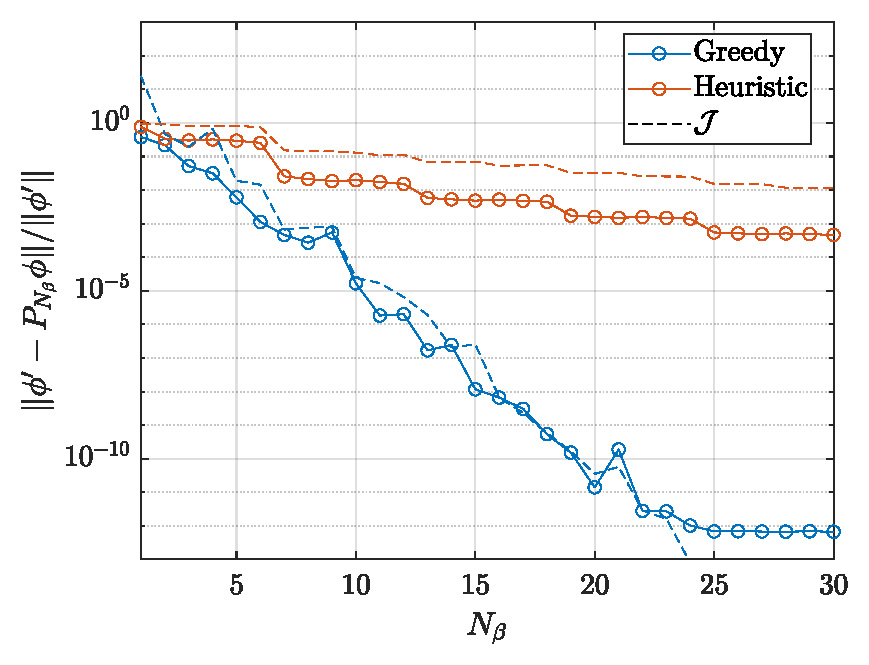
\includegraphics[width=1\linewidth]{figures/Oblique_Err_Obj_P.pdf}
        \caption{OWNS-P}\label{fig:oblique-err-p}
    \end{subfigure}
    \begin{subfigure}[b]{0.48\textwidth}
        \centering
        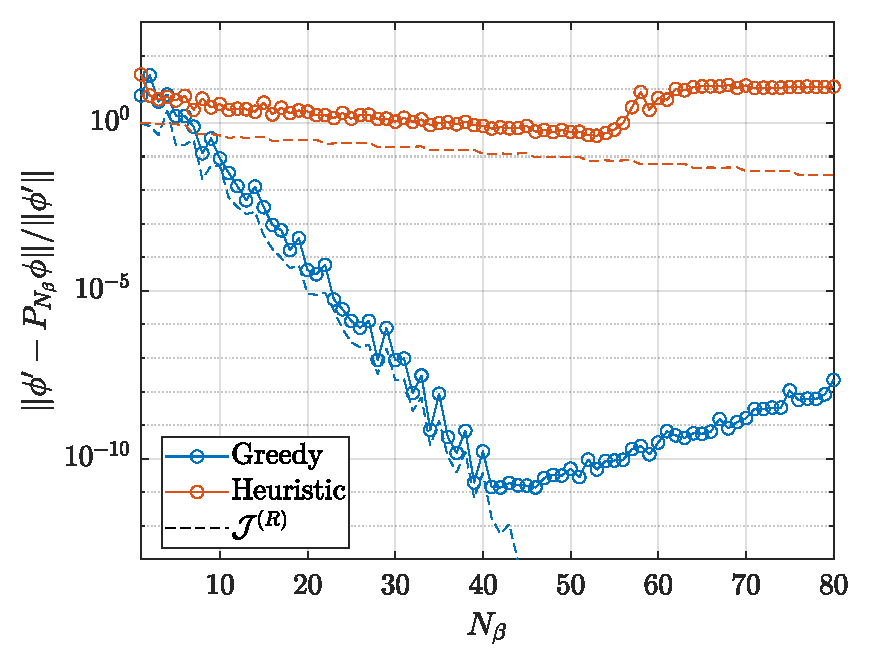
\includegraphics[width=1\linewidth]{figures/Oblique_Err_Obj_R.pdf}
        \caption{OWNS-R}\label{fig:oblique-err-r}
    \end{subfigure}
    \caption{Error convergence as a function of $N_\beta$ for OWNS-P and OWNS-R for the low-speed oblique wave case.}
    \label{fig:oblique-err}
\end{figure}


\subsection{2D high-speed boundary-layer flow}

We consider the Mach 4.5 boundary-layer flow over an adiabatic flat plate studied by Ma and Zhong~\cite{Ma_2003_DNS_1}, which was used by Zhu and Towne~\cite{Zhu_2021_OWNS-R} as a validation case for the OWNS-R formulation. The flow conditions are $M_\infty = 4.5$, $T_\infty^*=65.15$ K, $p_\infty^*=728.44$ Pa, $Pr=0.72$, and unit Reynolds number $Re_\infty^* = \rho_\infty^* U_\infty^* / \mu_\infty^*=7.2\times10^6 / $ m. Figure~\ref{fig:zhong-err} shows the convergence of the error as a function of $N_\beta$ for OWNS-P and OWNS-R. We again observe that OWNS-P achieves machine zero error, while OWNS-R does not. We also highlight that for OWNS-R only, we excluded downstream-going eigenvalues with $\alpha_i>100$ from the selection procedure, which improve the accuracy of the approximation. Excluding these modes does not significantly affect the accuracy of the approximation because they decay rapidly.

\begin{figure}
    \centering
    \begin{subfigure}[b]{0.48\textwidth}
        \centering
        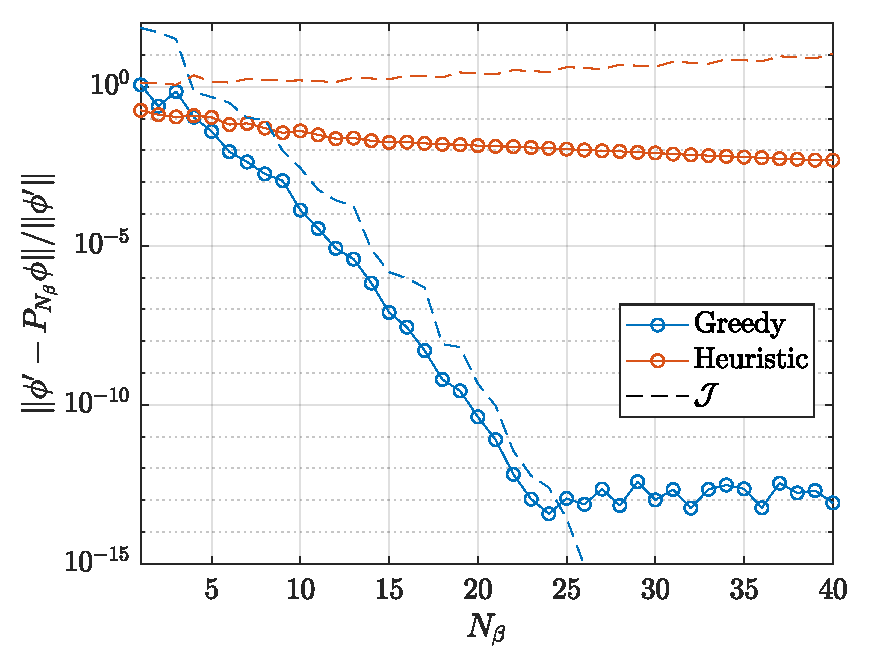
\includegraphics[width=1\linewidth]{figures/Zhong-OWNS-P.pdf}
        \caption{OWNS-P}
        \label{fig:zhong-err-p}
    \end{subfigure}
    \begin{subfigure}[b]{0.48\textwidth}
        \centering
        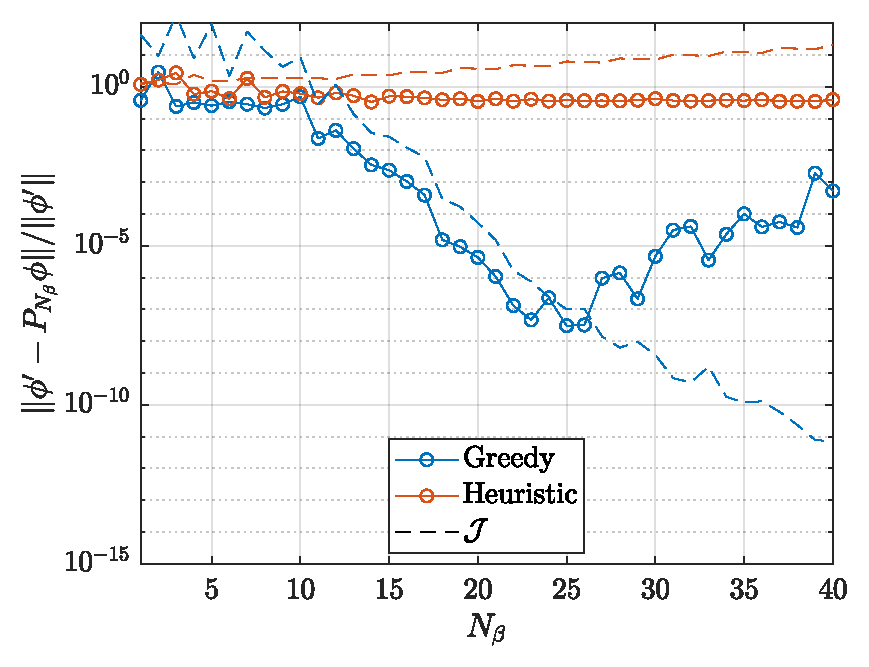
\includegraphics[width=1\linewidth]{figures/Zhong-OWNS-R.pdf}
        \caption{OWNS-R}
        \label{fig:zhong-err-r}
    \end{subfigure}\\
    \caption{Convergence of the error for greedy and heuristic parameter selection for 2D high-speed boundary-layer flow.}
    \label{fig:zhong-err}
\end{figure}



\subsection{2D mixing-layer flow}

To demonstrate broader applicability of the greedy approach, we consider a 2D mixing layer as our final test case. We consider a linearized version of the case studied by Colonius et al.~\cite{Colonius_1997_ML}. The fast stream Mach number is $M_1 = 0.5$, while the slow-stream is $M_2=0.25$. We introduce the vorticity thickness
\begin{equation}
    \delta^* = \Big(\frac{U_1^* - U_2^*}{|\partial U^* / \partial y^* |_{\max}}\Big)_{x^* = x_0^*},
\end{equation}
and specify a Reynolds number of $Re = \rho_\infty^* (U_2^* - U_1^*) \delta ^* / \mu_\infty^*=250$. The temperatures of the two free streams are equal, while the fluid properties ($\mu^*$ and $k^*$) are taken to be constant, while $Pr=1$ and $\gamma=1.4$.

We apply the greedy algorithm at the inlet, and observe 

that the objective function converges reasonable quickly for both greedy and heuristic parameter selection, for both OWNS-R and OWNS-P, as shown in figure~\ref{fig:mixing-obj}. Figure~\ref{fig:mixing-obj-pm} splits the objective function into upstream- and downstream-going components. Whereas for boundary-layer flows, $\hat{J}_+$ increases with increasing $N_\beta$, we have that both $\hat{J}_+$ and $\hat{J}_-$ decrease with increasing $N_\beta$ for the mixing layer, which explains the better convergence of the OWNS-R objective function for this flow. We take a random linear combination of the eigenvectors of $M$ and compute the error in the projection as $N_\beta$ increases, plotted in figure~\ref{fig:mixing-err}. For OWNS-P, we see that machine zero precision is obtained around $N_\beta=29$ with greedy parameter selection, while the error is several orders of magnitude larger for heuristic selection. In contrast, greedy selection for OWNS-R approaches machine zero around $N_\beta=50$, but increases again with increasing $N_\beta$ due to the error in the computation of $\beta_*^j$. 

Figure~\ref{fig:mixing-params} shows the recursion parameters chosen using the heuristic and greedy selection approaches. As discussed by Towne and Colonius~\cite{Towne_2015_OWNS-O}, the filter converges when $\beta_-^j$ are closer to the upstream-going eigenvalues than $\beta_+^j$, and vice versa. Therefore, the greedy approach preferentially places the recursion parameters closer to the interface between the upstream- and downstream-going branches. We note that the upstream- and downstream-going branches are further separated in the mixing layer than in the boundary layer, which is why the filter converges more quickly.


\begin{figure}
    \centering
    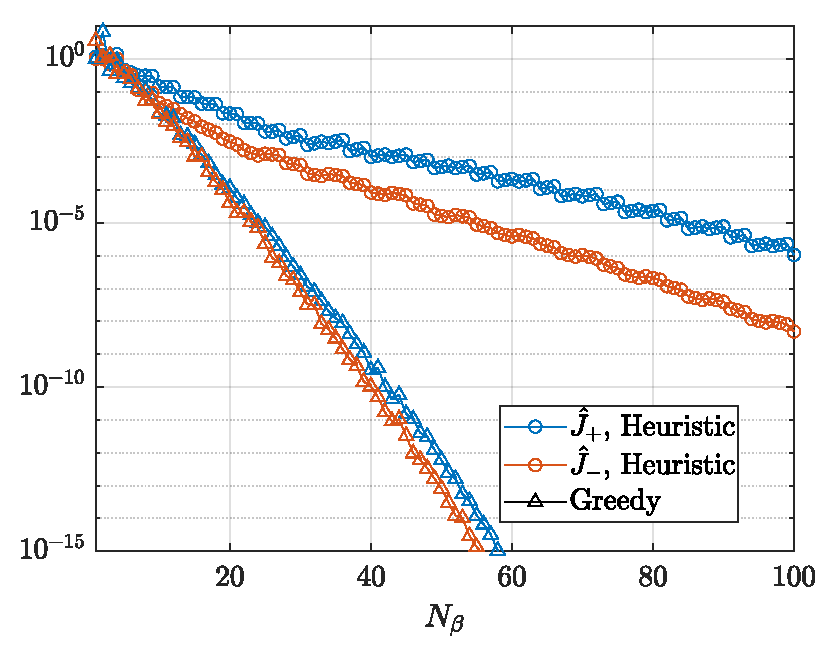
\includegraphics[width=0.5\linewidth]{figures/Mixing_Obj_R_pm.pdf}
    \caption{Convergence of the objective function, split into upstream- and downstream-going components, for greedy and heuristic parameter selection for the mixing layer flow}
    \label{fig:mixing-obj-pm}
\end{figure}

\begin{figure}
    \centering
    \begin{subfigure}[b]{0.48\textwidth}
        \centering
        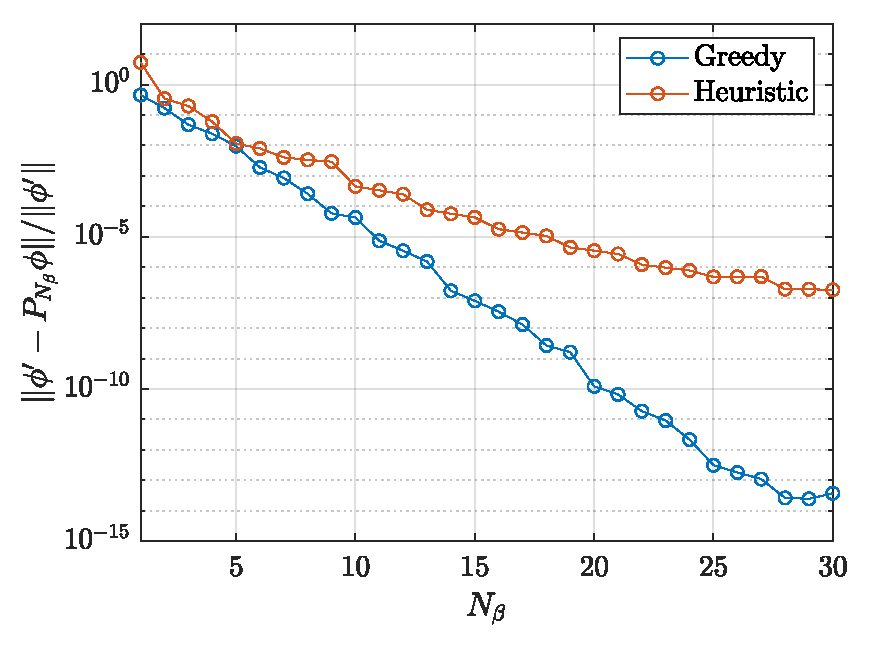
\includegraphics[width=1\linewidth]{figures/Mixing_Err_P.pdf}
        \caption{OWNS-P}
        \label{fig:mixing-err-p}
    \end{subfigure}
    \begin{subfigure}[b]{0.48\textwidth}
        \centering
        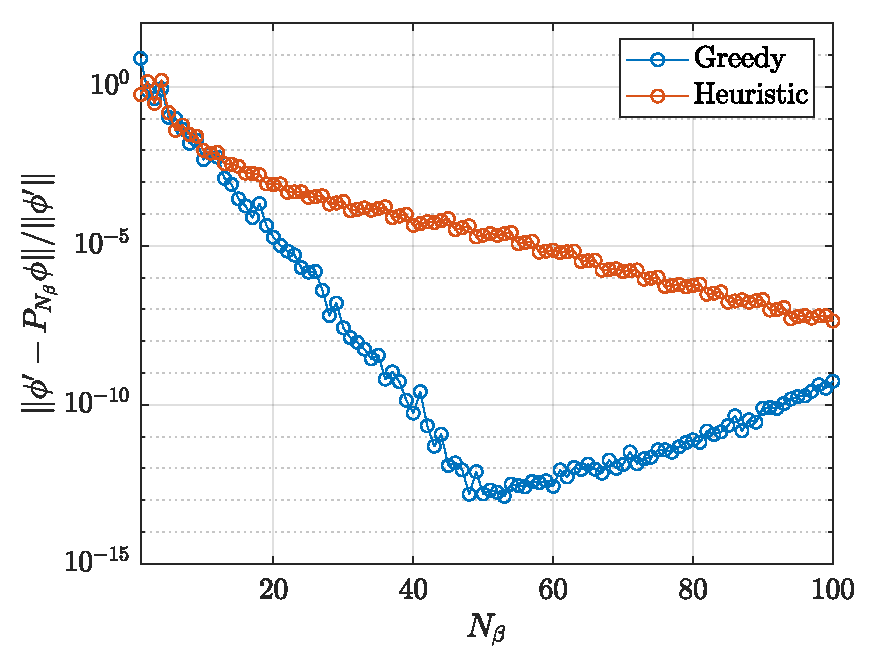
\includegraphics[width=1\linewidth]{figures/Mixing_Err_R.pdf}
        \caption{OWNS-R}
        \label{fig:mixing-err-r}
    \end{subfigure}\\
        \centering
    \begin{subfigure}[b]{0.48\textwidth}
        \centering
        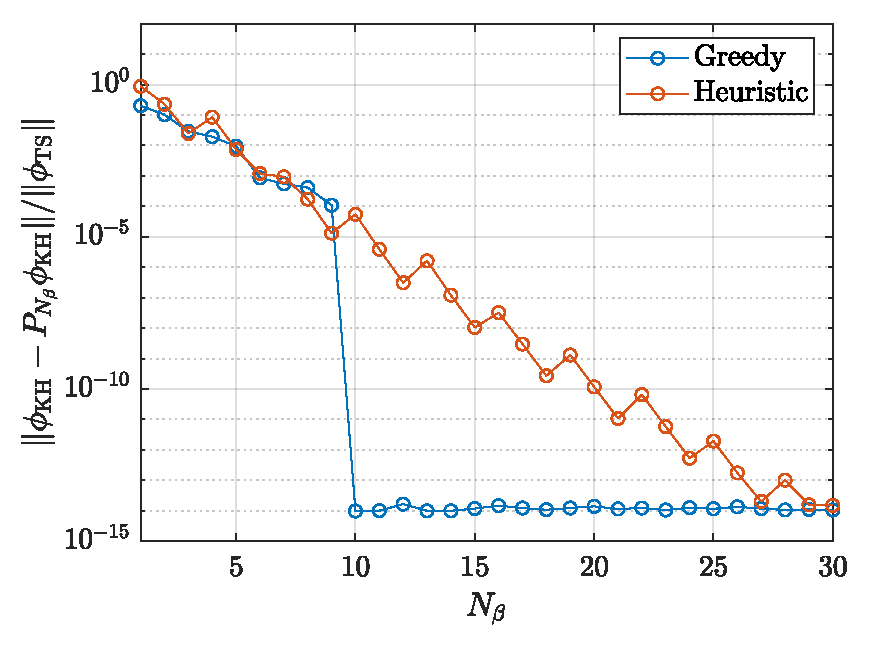
\includegraphics[width=1\linewidth]{figures/Mixing_Err_KH_P.pdf}
        \caption{OWNS-P, KH only}
        \label{fig:mixing-err-kh-p}
    \end{subfigure}
    \begin{subfigure}[b]{0.48\textwidth}
        \centering
        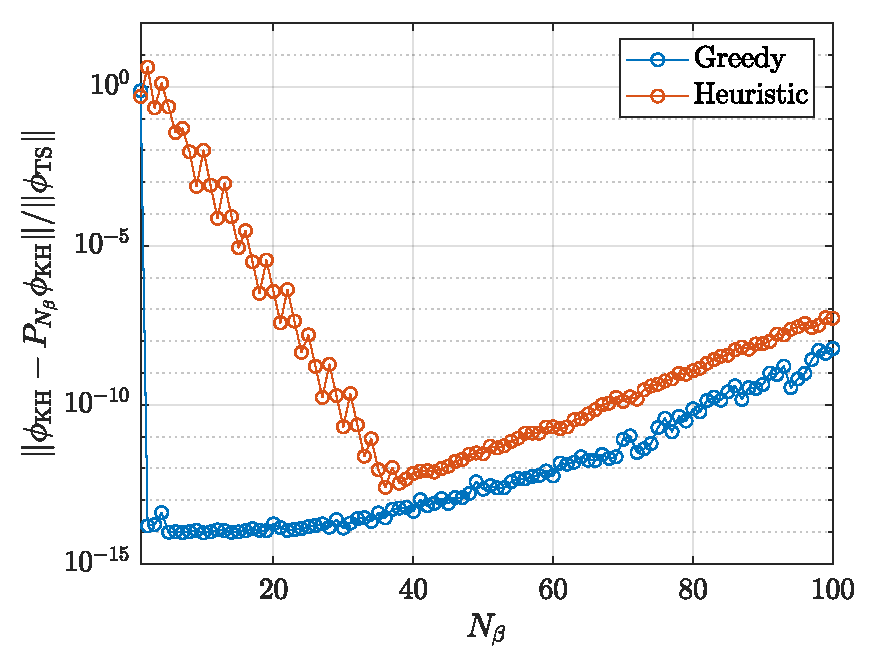
\includegraphics[width=1\linewidth]{figures/Mixing_Err_KH_R.pdf}
        \caption{OWNS-R, KH only}
        \label{fig:mixing-err-kh-r}
    \end{subfigure}
    \caption{Convergence of the error for greedy and heuristic parameter selection for mixing layer.}
    \label{fig:mixing-err}
\end{figure}

\begin{figure}
    \centering
    \begin{subfigure}[b]{0.48\textwidth}
        \centering
        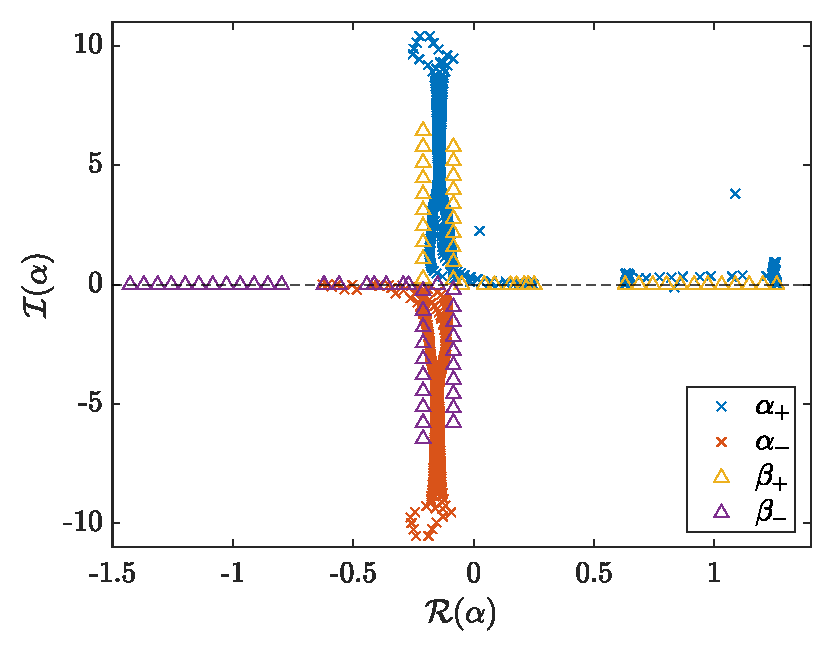
\includegraphics[width=1\linewidth]{figures/Mixing_Params_Heuristic.pdf}
        \caption{Heuristic}
        \label{fig:mixing-params-heuristic}
    \end{subfigure}
    \begin{subfigure}[b]{0.48\textwidth}
        \centering
        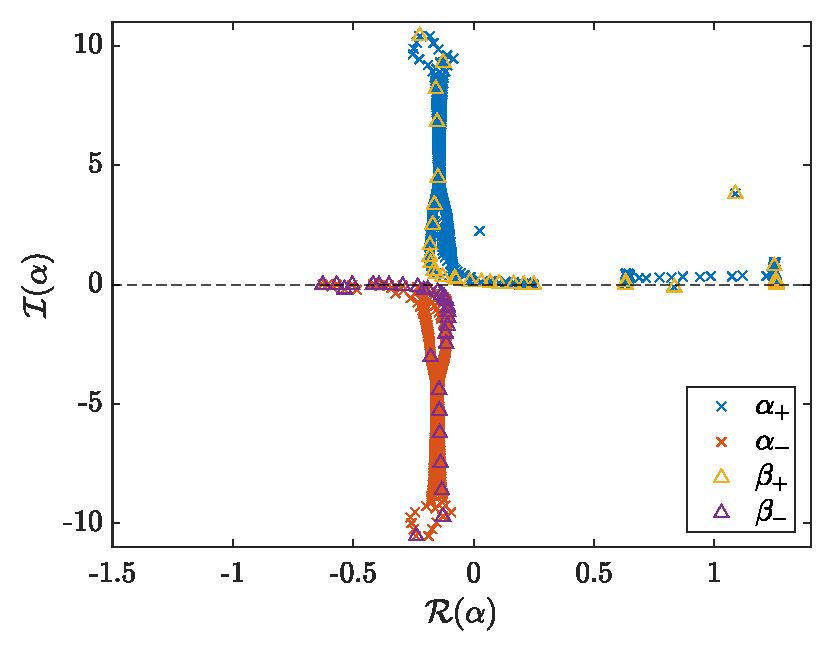
\includegraphics[width=1\linewidth]{figures/Mixing_Params_Greedy.pdf}
        \caption{Greedy}
        \label{fig:mixing-params-greedy}
    \end{subfigure}
    \caption{Recursion parameter selection for mixing layer.}
    \label{fig:mixing-params}
\end{figure}